\documentclass{article}
\usepackage[utf8]{inputenc}
\usepackage{indentfirst}
\usepackage{graphicx}

\begin{document}

\section{Oversampling e Undersampling}

Oversampling e Undersampling são técnicas de balanceamento de dados para problemas de classificação. Tais técnicas permitem que os algoritmos de machine learning onde as classes de um conjunto de dados são desbalanceadas não sejam influenciados pelo desequilíbrio presente entre as classes.
\\
Normalmente, em problemas de classificação que apresentam esse tipo de comportamento dos dados, a classe de maior interesse é a minoritária e por isso essa questão deve ser levada em consideração na construção do algoritmo.No caso do assunto abordado neste trabalho, encontramos exatamente essa situação, onde temos as classes fraude e não fraude, sendo a classe fraude a classe minoritária e de interesse.
\\

\section{Oversampling}
Oversampling consiste na técnica de duplicar as amostras da nossa classe minoritária. Caso essa técnica seja feita com amostras aleatórias, pode ocasionar o efeito chamado de overfitting, nesse caso, apresentaremos soluções para evitar esse problema.
\section{Undersampling}
Undersampling utiliza a exclusão de amostras da classe majoritária, essa técnica pode apresentar a perda de informações importantes em nosso conjunto de dados, criando um viés para o algoritmo.
\\
\section{SMOTE(Synthetic Minority Oversampling Technique)}
SMOTE é uma técnica de oversampling, onde são geradas amostras sintéticas para a classe minoritária, essa técnica ajuda a evitar o overfitting quando comparada com a utilização do oversampling somente com amostras aleatórias.Tal técnica, consiste em selecionar uma amostra aleatória e em seguida, obter k vizinhos próximos para essa instância. Então, N vizinhos são selecionados aleatoriamente e a amostra é criada em um ponto entre a instaância original e seu vizinho escolhido.

\begin{figure}[h]
\caption{Exemplificação da técnica SMOTE}

\centering % para centralizarmos a figura
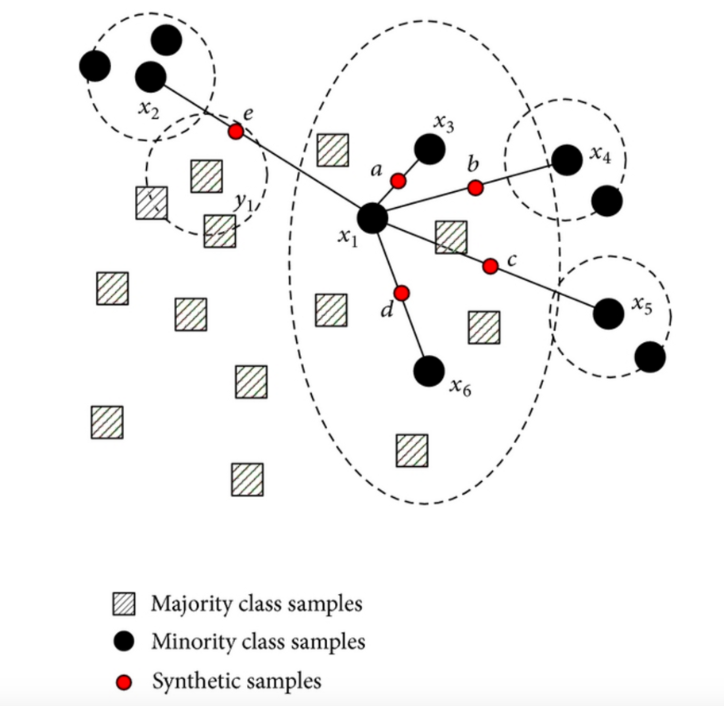
\includegraphics[width=10cm]{images/SMOTE-img.png} % leia abaixo
\label{figura:smote}
\end{figure}

\end{document}
